% -----------------------------*- LaTeX -*------------------------------
\documentclass[12pt]{report}
\usepackage{sparsity_structures_and_algorithms_10, epsfig}
\usepackage{amsmath}
% Use something like:
% % Use something like:
% % Use something like:
% \input{../../macros}

% groupings of objects.
\newcommand{\set}[1]{\left\{ #1 \right\}}
\newcommand{\seq}[1]{\left(#1\right)}
\newcommand{\ang}[1]{\langle#1\rangle}
\newcommand{\tuple}[1]{\left(#1\right)}

% numerical shortcuts.
\newcommand{\abs}[1]{\left| #1\right|}
\newcommand{\floor}[1]{\left\lfloor #1 \right\rfloor}
\newcommand{\ceil}[1]{\left\lceil #1 \right\rceil}

% linear algebra shortcuts.
\newcommand{\change}{\Delta}
\newcommand{\norm}[1]{\left\| #1\right\|}
\newcommand{\dprod}[1]{\langle#1\rangle}
\newcommand{\linspan}[1]{\langle#1\rangle}
\newcommand{\conj}[1]{\overline{#1}}
\newcommand{\gradient}{\nabla}
\newcommand{\der}{\frac{d}{dx}}
\newcommand{\lap}{\Delta}
\newcommand{\kron}{\otimes}
\newcommand{\nperp}{\nvdash}

\newcommand{\mat}[1]{\left( \begin{smallmatrix}#1 \end{smallmatrix} \right)}

% derivatives and limits
\newcommand{\partder}[2]{\frac{\partial #1}{\partial #2}}
\newcommand{\partdern}[3]{\frac{\partial^{#3} #1}{\partial #2^{#3}}}

% Arrows
\newcommand{\diverge}{\nearrow}
\newcommand{\notto}{\nrightarrow}
\newcommand{\up}{\uparrow}
\newcommand{\down}{\downarrow}
% gets and gives are defined!

% ordering operators
\newcommand{\oleq}{\preceq}
\newcommand{\ogeq}{\succeq}

% programming and logic operators
\newcommand{\dfn}{:=}
\newcommand{\assign}{:=}
\newcommand{\co}{\ co\ }
\newcommand{\en}{\ en\ }


% logic operators
\newcommand{\xor}{\oplus}
\newcommand{\Land}{\bigwedge}
\newcommand{\Lor}{\bigvee}
\newcommand{\finish}{$\Box$}
\newcommand{\contra}{\Rightarrow \Leftarrow}
\newcommand{\iseq}{\stackrel{_?}{=}}


% Set theory
\newcommand{\symdiff}{\Delta}
\newcommand{\union}{\cup}
\newcommand{\inters}{\cap}
\newcommand{\Union}{\bigcup}
\newcommand{\Inters}{\bigcap}
\newcommand{\nullSet}{\phi}

% graph theory
\newcommand{\nbd}{\Gamma}

% Script alphabets
% For reals, use \Re

% greek letters
\newcommand{\eps}{\epsilon}
\newcommand{\del}{\delta}
\newcommand{\ga}{\alpha}
\newcommand{\gb}{\beta}
\newcommand{\gd}{\del}
\newcommand{\gf}{\phi}
\newcommand{\gF}{\Phi}
\newcommand{\gl}{\lambda}
\newcommand{\gm}{\mu}
\newcommand{\gn}{\nu}
\newcommand{\gr}{\rho}
\newcommand{\gs}{\sigma}
\newcommand{\gt}{\theta}
\newcommand{\gx}{\xi}

\newcommand{\sw}{\sigma}
\newcommand{\SW}{\Sigma}
\newcommand{\ew}{\lambda}
\newcommand{\EW}{\Lambda}

\newcommand{\Del}{\Delta}
\newcommand{\gD}{\Delta}
\newcommand{\gG}{\Gamma}
\newcommand{\gO}{\Omega}
\newcommand{\gL}{\Lambda}
\newcommand{\gS}{\Sigma}

% Formatting shortcuts
\newcommand{\red}[1]{\textcolor{red}{#1}}
\newcommand{\blue}[1]{\textcolor{blue}{#1}}
\newcommand{\htext}[2]{\texorpdfstring{#1}{#2}}

% Statistics
\newcommand{\distr}{\sim}
\newcommand{\stddev}{\sigma}
\newcommand{\covmatrix}{\Sigma}
\newcommand{\mean}{\mu}
\newcommand{\param}{\gt}
\newcommand{\ftr}{\phi}

% General utility
\newcommand{\todo}[1]{\footnote{TODO: #1}}
\newcommand{\exclaim}[1]{{\textbf{\textit{#1}}}}
\newcommand{\tbc}{[\textbf{Incomplete}]}
\newcommand{\chk}{[\textbf{Check}]}
\newcommand{\oprob}{[\textbf{OP}]:}
\newcommand{\core}[1]{\textbf{Core Idea:}}
\newcommand{\why}{[\textbf{Find proof}]}
\newcommand{\opt}[1]{\textit{#1}}


\DeclareMathOperator*{\argmin}{arg\,min}
\DeclareMathOperator{\rank}{rank}
\newcommand{\redcol}[1]{\textcolor{red}{#1}}
\newcommand{\bluecol}[1]{\textcolor{blue}{#1}}
\newcommand{\greencol}[1]{\textcolor{green}{#1}}


\renewcommand{\~}{\htext{$\sim$}{~}}


% groupings of objects.
\newcommand{\set}[1]{\left\{ #1 \right\}}
\newcommand{\seq}[1]{\left(#1\right)}
\newcommand{\ang}[1]{\langle#1\rangle}
\newcommand{\tuple}[1]{\left(#1\right)}

% numerical shortcuts.
\newcommand{\abs}[1]{\left| #1\right|}
\newcommand{\floor}[1]{\left\lfloor #1 \right\rfloor}
\newcommand{\ceil}[1]{\left\lceil #1 \right\rceil}

% linear algebra shortcuts.
\newcommand{\change}{\Delta}
\newcommand{\norm}[1]{\left\| #1\right\|}
\newcommand{\dprod}[1]{\langle#1\rangle}
\newcommand{\linspan}[1]{\langle#1\rangle}
\newcommand{\conj}[1]{\overline{#1}}
\newcommand{\gradient}{\nabla}
\newcommand{\der}{\frac{d}{dx}}
\newcommand{\lap}{\Delta}
\newcommand{\kron}{\otimes}
\newcommand{\nperp}{\nvdash}

\newcommand{\mat}[1]{\left( \begin{smallmatrix}#1 \end{smallmatrix} \right)}

% derivatives and limits
\newcommand{\partder}[2]{\frac{\partial #1}{\partial #2}}
\newcommand{\partdern}[3]{\frac{\partial^{#3} #1}{\partial #2^{#3}}}

% Arrows
\newcommand{\diverge}{\nearrow}
\newcommand{\notto}{\nrightarrow}
\newcommand{\up}{\uparrow}
\newcommand{\down}{\downarrow}
% gets and gives are defined!

% ordering operators
\newcommand{\oleq}{\preceq}
\newcommand{\ogeq}{\succeq}

% programming and logic operators
\newcommand{\dfn}{:=}
\newcommand{\assign}{:=}
\newcommand{\co}{\ co\ }
\newcommand{\en}{\ en\ }


% logic operators
\newcommand{\xor}{\oplus}
\newcommand{\Land}{\bigwedge}
\newcommand{\Lor}{\bigvee}
\newcommand{\finish}{$\Box$}
\newcommand{\contra}{\Rightarrow \Leftarrow}
\newcommand{\iseq}{\stackrel{_?}{=}}


% Set theory
\newcommand{\symdiff}{\Delta}
\newcommand{\union}{\cup}
\newcommand{\inters}{\cap}
\newcommand{\Union}{\bigcup}
\newcommand{\Inters}{\bigcap}
\newcommand{\nullSet}{\phi}

% graph theory
\newcommand{\nbd}{\Gamma}

% Script alphabets
% For reals, use \Re

% greek letters
\newcommand{\eps}{\epsilon}
\newcommand{\del}{\delta}
\newcommand{\ga}{\alpha}
\newcommand{\gb}{\beta}
\newcommand{\gd}{\del}
\newcommand{\gf}{\phi}
\newcommand{\gF}{\Phi}
\newcommand{\gl}{\lambda}
\newcommand{\gm}{\mu}
\newcommand{\gn}{\nu}
\newcommand{\gr}{\rho}
\newcommand{\gs}{\sigma}
\newcommand{\gt}{\theta}
\newcommand{\gx}{\xi}

\newcommand{\sw}{\sigma}
\newcommand{\SW}{\Sigma}
\newcommand{\ew}{\lambda}
\newcommand{\EW}{\Lambda}

\newcommand{\Del}{\Delta}
\newcommand{\gD}{\Delta}
\newcommand{\gG}{\Gamma}
\newcommand{\gO}{\Omega}
\newcommand{\gL}{\Lambda}
\newcommand{\gS}{\Sigma}

% Formatting shortcuts
\newcommand{\red}[1]{\textcolor{red}{#1}}
\newcommand{\blue}[1]{\textcolor{blue}{#1}}
\newcommand{\htext}[2]{\texorpdfstring{#1}{#2}}

% Statistics
\newcommand{\distr}{\sim}
\newcommand{\stddev}{\sigma}
\newcommand{\covmatrix}{\Sigma}
\newcommand{\mean}{\mu}
\newcommand{\param}{\gt}
\newcommand{\ftr}{\phi}

% General utility
\newcommand{\todo}[1]{\footnote{TODO: #1}}
\newcommand{\exclaim}[1]{{\textbf{\textit{#1}}}}
\newcommand{\tbc}{[\textbf{Incomplete}]}
\newcommand{\chk}{[\textbf{Check}]}
\newcommand{\oprob}{[\textbf{OP}]:}
\newcommand{\core}[1]{\textbf{Core Idea:}}
\newcommand{\why}{[\textbf{Find proof}]}
\newcommand{\opt}[1]{\textit{#1}}


\DeclareMathOperator*{\argmin}{arg\,min}
\DeclareMathOperator{\rank}{rank}
\newcommand{\redcol}[1]{\textcolor{red}{#1}}
\newcommand{\bluecol}[1]{\textcolor{blue}{#1}}
\newcommand{\greencol}[1]{\textcolor{green}{#1}}


\renewcommand{\~}{\htext{$\sim$}{~}}


% groupings of objects.
\newcommand{\set}[1]{\left\{ #1 \right\}}
\newcommand{\seq}[1]{\left(#1\right)}
\newcommand{\ang}[1]{\langle#1\rangle}
\newcommand{\tuple}[1]{\left(#1\right)}

% numerical shortcuts.
\newcommand{\abs}[1]{\left| #1\right|}
\newcommand{\floor}[1]{\left\lfloor #1 \right\rfloor}
\newcommand{\ceil}[1]{\left\lceil #1 \right\rceil}

% linear algebra shortcuts.
\newcommand{\change}{\Delta}
\newcommand{\norm}[1]{\left\| #1\right\|}
\newcommand{\dprod}[1]{\langle#1\rangle}
\newcommand{\linspan}[1]{\langle#1\rangle}
\newcommand{\conj}[1]{\overline{#1}}
\newcommand{\gradient}{\nabla}
\newcommand{\der}{\frac{d}{dx}}
\newcommand{\lap}{\Delta}
\newcommand{\kron}{\otimes}
\newcommand{\nperp}{\nvdash}

\newcommand{\mat}[1]{\left( \begin{smallmatrix}#1 \end{smallmatrix} \right)}

% derivatives and limits
\newcommand{\partder}[2]{\frac{\partial #1}{\partial #2}}
\newcommand{\partdern}[3]{\frac{\partial^{#3} #1}{\partial #2^{#3}}}

% Arrows
\newcommand{\diverge}{\nearrow}
\newcommand{\notto}{\nrightarrow}
\newcommand{\up}{\uparrow}
\newcommand{\down}{\downarrow}
% gets and gives are defined!

% ordering operators
\newcommand{\oleq}{\preceq}
\newcommand{\ogeq}{\succeq}

% programming and logic operators
\newcommand{\dfn}{:=}
\newcommand{\assign}{:=}
\newcommand{\co}{\ co\ }
\newcommand{\en}{\ en\ }


% logic operators
\newcommand{\xor}{\oplus}
\newcommand{\Land}{\bigwedge}
\newcommand{\Lor}{\bigvee}
\newcommand{\finish}{$\Box$}
\newcommand{\contra}{\Rightarrow \Leftarrow}
\newcommand{\iseq}{\stackrel{_?}{=}}


% Set theory
\newcommand{\symdiff}{\Delta}
\newcommand{\union}{\cup}
\newcommand{\inters}{\cap}
\newcommand{\Union}{\bigcup}
\newcommand{\Inters}{\bigcap}
\newcommand{\nullSet}{\phi}

% graph theory
\newcommand{\nbd}{\Gamma}

% Script alphabets
% For reals, use \Re

% greek letters
\newcommand{\eps}{\epsilon}
\newcommand{\del}{\delta}
\newcommand{\ga}{\alpha}
\newcommand{\gb}{\beta}
\newcommand{\gd}{\del}
\newcommand{\gf}{\phi}
\newcommand{\gF}{\Phi}
\newcommand{\gl}{\lambda}
\newcommand{\gm}{\mu}
\newcommand{\gn}{\nu}
\newcommand{\gr}{\rho}
\newcommand{\gs}{\sigma}
\newcommand{\gt}{\theta}
\newcommand{\gx}{\xi}

\newcommand{\sw}{\sigma}
\newcommand{\SW}{\Sigma}
\newcommand{\ew}{\lambda}
\newcommand{\EW}{\Lambda}

\newcommand{\Del}{\Delta}
\newcommand{\gD}{\Delta}
\newcommand{\gG}{\Gamma}
\newcommand{\gO}{\Omega}
\newcommand{\gL}{\Lambda}
\newcommand{\gS}{\Sigma}

% Formatting shortcuts
\newcommand{\red}[1]{\textcolor{red}{#1}}
\newcommand{\blue}[1]{\textcolor{blue}{#1}}
\newcommand{\htext}[2]{\texorpdfstring{#1}{#2}}

% Statistics
\newcommand{\distr}{\sim}
\newcommand{\stddev}{\sigma}
\newcommand{\covmatrix}{\Sigma}
\newcommand{\mean}{\mu}
\newcommand{\param}{\gt}
\newcommand{\ftr}{\phi}

% General utility
\newcommand{\todo}[1]{\footnote{TODO: #1}}
\newcommand{\exclaim}[1]{{\textbf{\textit{#1}}}}
\newcommand{\tbc}{[\textbf{Incomplete}]}
\newcommand{\chk}{[\textbf{Check}]}
\newcommand{\oprob}{[\textbf{OP}]:}
\newcommand{\core}[1]{\textbf{Core Idea:}}
\newcommand{\why}{[\textbf{Find proof}]}
\newcommand{\opt}[1]{\textit{#1}}


\DeclareMathOperator*{\argmin}{arg\,min}
\DeclareMathOperator{\rank}{rank}
\newcommand{\redcol}[1]{\textcolor{red}{#1}}
\newcommand{\bluecol}[1]{\textcolor{blue}{#1}}
\newcommand{\greencol}[1]{\textcolor{green}{#1}}


\renewcommand{\~}{\htext{$\sim$}{~}}

\begin{document}

% \course{EE 381V}			% optional
% \coursetitle{Sparsity, Structures and Algorithms} % optional
% \semester{Spring 2010}			% optional
% \lecturer{Sujay Sanghavi}		% optional
\scribe{vishvAs vAsuki, Praneeth Netrapalli}		% required
\lecturenumber{20}			% required, must be a number
\lecturedate{March 31}		% required, omit year

\maketitle

% ----------------------------------------------------------------------

\section{Topics covered}
\begin{itemize}
\item Sparse Representation in Over Complete Basis
\item Finding Sparse Representation using $\ell_1$ minimization
\end{itemize}

\section{Sparse representation in overcomplete basis}
\subsection{Motivation from digital signal processing}
Let $\Phi$ be a matrix whose columns are composed of the basis functions/ vectors for the frequency domain. Let $\Psi$ be a matrix similarly formed using the basis functions/ vectors for the time domain.

Consider the signal shown in figure \ref{fig:signalExample}. We have added together two signals with sparse representations in $\Phi$ and $\Psi$ alone to produce a signal which is sparse in neither. In other words, this resultant signal does not have a sparse representation in $\Phi$ alone or in $\Psi$ alone. But, it can be seen to have a sparse representation in $\Phi$ and $\Psi$ together.

It must be noted, however that the columns of $[\Phi\ \Psi]$ are not linearly independent. So, $[\Phi\ \Psi]$ forms an 'overcomplete basis'. This motivates the following problem.

\subsection{Problem}
Given a signal (or a vector x in general), when can we find a sparse representation in the 'overcomplete basis' $[\Phi\ \Psi]$?

\subsubsection{Ill posedness/ non-uniqueness}
There are an infinite number of representations for any signal in a pair of bases. Looking for sparsity in representation may help, but this is not enough to guarantee uniqueness.

To see this, consider a basis $\Psi$ which differs from $\Phi$ in only two basis vectors, but is the same as $\Phi$ otherwise. Then, sparsity of x in $\Psi$ is equivalent to sparsity in $\Phi$; and it is even hard for an x which is sparse in $\Psi$ or $\Phi$ alone, to have a unique representation in the overcomplete basis $[\Phi\ \Psi]$. For example, suppose that both $\Phi$ and $\Psi$ include the basis vectors $\set{\phi_1, \phi_2}$, and consider $x = \phi_1 + \phi_2$. x has an infinite number of sparse representations in the basis $[\Phi\ \Psi]$.

So, we must add an additional condition: $\Phi$ and $\Psi$ must be 'different' enough. This property is usually referred to as 'incoherence'.

\begin{figure}
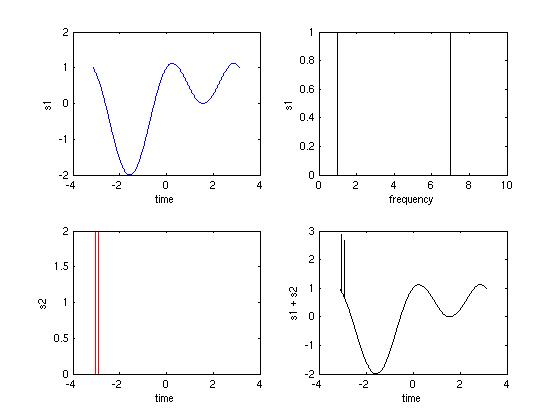
\includegraphics[scale = 0.75]{signalExampleMatlab.jpg}
\caption{The signal s1 has a sparse representation in the frequency domain. s2 has a sparse representation in the time domain. But, the signal (s1 + s2) has a sparse repersentation in an overcompelte basis, but not in either the frequency or time domain alone.}
\label{fig:signalExample}
\end{figure}

\subsection{Basic uncertainty principle}
\begin{theorem}
Let $\Phi$ and $\Psi$ be two orthonormal bases for a vector space. For any vector $s \neq 0$, let $s = \Phi a$ and $s = \Psi b$. Let M = $\max_{i,j}|\dprod{\gf_i, \psi_j}|$. Then:
$$\frac{\norm{a}_0 + \norm{b}_0}{2} \geq \sqrt{\norm{a}_0\norm{b}_0} \geq M^{-1}$$.
\end{theorem}
\begin{proof}
The first inequality comes from the well known AM-GM inequality, so we prove $\sqrt{\norm{a}_0\norm{b}_0} \geq M^{-1}$.

Without loss of generality, suppose that $s^{T}s = 1$.

$$1 = a^{T}\Phi^{T}\Psi b \leq \sum_{i,j} |a_i||\dprod{\gf_i, \psi_j}||b_j| \leq M\sum_i |a_i| \sum_j |b_j|$$

Let $A = \norm{a}_0, B = \norm{b}_0$. From $s^{T}s = 1$, we have that $\sum_i |a_i|^{2} = 1 = \sum_i |b_i|^{2}$. Also, $\forall i: |a_i| \leq 1, |b_i| \leq 1$. So:
 
$$\sum_i |a_i| \leq \sqrt{A}, \sum_i |b_i| \leq \sqrt{B}$$

Substituting this into the earlier inequality, we have $\sqrt{\norm{a}_0\norm{b}_0} \geq M^{-1}$.
\end{proof}

From this, we have the following theorem, whose proof is left as a homework exercise.

\begin{theorem}
If $s = [\Phi\ \Psi]g_1, s = [\Phi\ \Psi]g_2$, then $\norm{g_1}_0 + \norm{g_2}_0 \geq \frac{2}{M}$.
\end{theorem}

From this, we have the following corollary:
\begin{corollary}
Suppose that $s = [\Phi\ \Psi]g_1$, and $\norm{g_1}_0 < M^{-1}$. Then, there does not exist a $g_2$ such that $s = [\Phi\ \Psi]g_2$ and $\norm{g_2}_0 < M^{-1}$.
\end{corollary}


Incoherence is the situation where M is small. Thus, incoherence ensures uniqueness for the sparsest representation. In other words, any other representation will have more non-zeros.

This motivates the following question: If s has a unique sparse representation, how do we find it? The answer to this is explored in the next section.


\section{Sparse Representation using $\ell_1$ minimization}
Suppose we want to find the sparsest $\gamma$ such that $\left[ \Phi \Psi \right] \gamma \; = \; s$.
The set of all feasible $\gamma$ is an affine subspace of $\mathbb{R}^n$. We want to know when
$\ell_1$ minimization gives us the sparsest solution.

\begin{theorem}[Donoho and Huo]
\label{DonohoHuo}
 If $\lVert\gamma\rVert_0 \; < \; \frac{1}{2}(1+\frac{1}{M})$ then $\|\widetilde{\gamma}\|_1 > \|\gamma\|_1$ for all
$\widetilde{\gamma}$ such that $\left[ \Phi \Psi \right] \widetilde{\gamma} = \left[ \Phi \Psi \right] \gamma$
\end{theorem}

\begin{proof}
Let $\|\gamma\|_0 \; < \; \frac{1}{2}(1+\frac{1}{M})$. Consider any
$\widetilde{\gamma}$ such that $\left[ \Phi \Psi \right] \widetilde{\gamma} = \left[ \Phi \Psi \right] \gamma$.
Let $x = \widetilde{\gamma} - \gamma$. Then, we have $\left[ \Phi \Psi \right] x = 0$.\\

$\|\widetilde{\gamma}\|_1 > \|\gamma\|_1$ \\ \\
$\Leftrightarrow \; \displaystyle\sum_{k \in \mbox{\begin{small} supp \end{small}}(\gamma)} \left( |\gamma_k + x_k| -|\gamma_k| \right) + \displaystyle\sum_{k \notin \mbox{\begin{small} supp \end{small}}(\gamma)} |x_k| > 0$\\ \\
$\Leftarrow \; \displaystyle\sum_{k \in \mbox{\begin{small} supp \end{small}}(\gamma)} -|x_k| + \displaystyle\sum_{k \notin \mbox{\begin{small} supp \end{small}}(\gamma)} |x_k| > 0$\\ \\
$\Leftrightarrow \; \frac{\displaystyle\sum_{\mbox{\begin{tiny} ON \end{tiny}}}|x_k|}{\displaystyle\sum_{\mbox{\begin{tiny} ALL \end{tiny}}}|x_k|} \; < \; \frac{1}{2}$\\

\noindent where $\displaystyle\sum_{\mbox{\begin{tiny} ON \end{tiny}}}|x_k| = \displaystyle\sum_{k \in \mbox{\begin{small} supp \end{small}}(\gamma)}|x_k|$ and
$\displaystyle\sum_{\mbox{\begin{tiny} ALL \end{tiny}}}|x_k| = \displaystyle\sum_k |x_k|$.\\

\noindent We want this to be true for all supports of size less than $\frac{1}{2}(1+\frac{1}{M})$ and for all $x$
such that $\left[ \Phi \Psi \right] x = 0$. Let $x\neq 0$ be any such vector and let $i$ be such that
$|x_i| \geq |x_j|$ for all $j$. WLOG, by rescaling, we can assume $x_i=v$ where $v$ is a fixed number.
For this, we have $\displaystyle\sum_{\mbox{\begin{tiny} ON \end{tiny}}}|x_k| \leq \|x\|_0 |v|$.

\begin{eqnarray*}
x = \left[ \begin{array}{r}
             x^\Phi \\
	     x^\Psi \\
            \end{array} \right]\\
\|x\|_1 = \|x^\Phi\|_1 + \|x^\Psi\|_1
\end{eqnarray*}

\noindent WLOG, say $i$ is in the $\Phi$ part.
\begin{eqnarray*}
\Phi x^\Phi = -\Psi x^\Psi \\
x^\Phi = -\Phi^T\Psi x^\Psi
\end{eqnarray*}
\noindent since $\Phi$ is an orthonormal matrix. So we have,
\begin{eqnarray*}
\begin{array}{rl}
      |v| = |x_i| &= | \left[ \Phi^T \Psi \right]_i x^\Psi| \\
		  & \leq M \|x^\Psi\|_1
\end{array}\\
\end{eqnarray*}
\begin{equation*}
 \Rightarrow \|x^\Psi\|_1 \; \geq  \; \frac{|v|}{M}
\end{equation*}

\noindent We also have,
\begin{eqnarray*}
\begin{array}{rl}
  \|x^\Phi\|_1 \; &\geq \; |v| \\ \\
  \Rightarrow \displaystyle\sum_{\mbox{\begin{tiny} ALL \end{tiny}}} |x_k| &= \; \|x\|_1 \; \geq \; |v|\left( 1 + \frac{1}{M}\right)
\end{array}
\end{eqnarray*}

\noindent So for any $x$ such that $\left[ \Phi \Psi \right] x = 0$,
\begin{equation*}
  \frac{\displaystyle\sum_{\mbox{\begin{tiny} ON \end{tiny}}}|x_k|}{\displaystyle\sum_{\mbox{\begin{tiny} ALL \end{tiny}}}|x_k|} \; \leq \; \frac{\|\gamma\|_0}{1+\frac{1}{M}}
\end{equation*}

\noindent and since $\|\gamma\|_0 < \frac{1}{2}\left(1+\frac{1}{M}\right)$, we have

\begin{equation*}
 \frac{\displaystyle\sum_{\mbox{\begin{tiny} ON \end{tiny}}}|x_k|}{\displaystyle\sum_{\mbox{\begin{tiny} ALL \end{tiny}}}|x_k|} \; < \; \frac{1}{2}
\end{equation*}

\noindent proving the result.

\end{proof}

Elad and Bruckstein further refine the sufficient condition to $\|\gamma\|_0 < \frac{\sqrt{2}-\frac{1}{2}}{M}$.
So under these conditions, if we solve $\operatorname{argmin}\; \|\gamma\|_1 \mbox{ s.t. } \left[ \Phi \Psi \right] \gamma=s$,
we are guaranteed to find the unique sparsest solution.

\end{document}

